\documentclass[12pt]{article}

\usepackage{natbib}
\usepackage{amsfonts, amsmath}
\usepackage{graphicx}
\usepackage{libertine}
\usepackage{fullpage}
\usepackage{hyperref}
\usepackage{booktabs}
\usepackage{array}
\usepackage{tabularx}
\usepackage{float}
\usepackage{placeins}
\usepackage{multirow}
\graphicspath{{graphics/}}

% Tighten float spacing to reduce whitespace gaps
\setlength{\floatsep}{4pt plus 1pt minus 1pt}
\setlength{\textfloatsep}{6pt plus 1pt minus 2pt}
\setlength{\intextsep}{4pt plus 1pt minus 1pt}
\setlength{\abovecaptionskip}{3pt}
\setlength{\belowcaptionskip}{1pt}
% Allow floats to take more of the page
\renewcommand{\topfraction}{0.95}
\renewcommand{\bottomfraction}{0.95}
\renewcommand{\textfraction}{0.05}
\renewcommand{\floatpagefraction}{0.90}

\hypersetup{
    colorlinks = true,
    linkcolor = blue,
    urlcolor  = blue,
    citecolor = blue,
    anchorcolor = blue}
\urlstyle{same}

\begin{document}

\title{Parameter Inference in a Stochastic SIR Epidemic Model on an Adaptive Network}
\author{}
\date{\today}
\maketitle

{\bf Group Composition:}
\begin{enumerate}
\item Maksymilian Paczyński, A0334580E, E1653593@u.nus.edu
\item Student 2, Student ID 2, email 2
\item Student 3, Student ID 3, email 3
\end{enumerate}

% ============================================================
\section{Introduction}
% ============================================================

We study parameter inference in a stochastic SIR epidemic model on an adaptive network \cite{GDB06}, where susceptible nodes can rewire away from infected contacts at rate $\rho$. The network begins as an Erdős–Rényi random graph $G(200, 0.05)$, yielding expected degree $\approx 10$ and connectivity with high probability \cite{Wik24}. The likelihood is intractable because the network co-evolves with the epidemic, so we apply Approximate Bayesian Computation (ABC). Three parameters are inferred from uniform priors:

\begin{table}[h]
\centering
\small
\begin{tabular}{clc}
\toprule
\textbf{Parameter} & \textbf{Meaning} & \textbf{Prior} \\
\midrule
$\beta$ & Infection probability per S--I edge per step & $\mathrm{Uniform}(0.05,\,0.50)$ \\
$\gamma$ & Recovery probability per infected node per step & $\mathrm{Uniform}(0.02,\,0.20)$ \\
$\rho$ & Rewiring probability per S--I edge per step & $\mathrm{Uniform}(0.0,\,0.8)$ \\
\bottomrule
\end{tabular}
\caption{Model parameters and priors.}
\end{table}

\noindent The epidemic peaks around $t \approx 10$--$13$ (infected fraction 0.6--0.8) and decays to near-zero by $t=200$. Each time step applies three sequential phases: Infection $\to$ Recovery $\to$ Rewiring. The observed dataset contains 40 replicate trajectories of infected fraction, rewiring counts, and the final degree histogram. All code and analysis scripts are available at: \url{https://github.com/[username]/[repo]} (to be updated before submission).

% ============================================================
\section{Rejection ABC}
% ============================================================

\subsection{Setup}

We run 10,000 prior simulations of the adaptive-network SIR model \cite{GDB06} ($N=200$, $p=0.05$, 5 initial infecteds, $T=200$ steps). For each simulation $i$, we compute a vector of summary statistics $\mathbf{s}_i$ and accept the parameter triple if the normalised Euclidean distance
\[
d_i = \left\| \frac{\mathbf{s}_i - \mathbf{s}^{\mathrm{obs}}}{\boldsymbol{\sigma}} \right\|_2
\]
falls within the $\varepsilon$-quantile of all distances ($\sigma_j$ = prior predictive std of statistic $j$). We evaluate $\varepsilon \in \{1\%, 5\%, 10\%, 20\%\}$; the primary criterion is $\varepsilon=5\%$ ($n=500$) \cite{PSP99}.

\subsection{Evaluation of Parameter Inference}
\label{sec:rejection}

Inference quality is assessed by three diagnostics: (i)~\textbf{marginal shrinkage} — how much the posterior contracts relative to the prior; (ii)~\textbf{tolerance robustness} — whether posteriors are stable across $\varepsilon$ levels; (iii)~\textbf{joint identifiability} — whether the $\beta$--$\rho$ posterior correlation $|r|$ remains below 0.3 (our identifiability threshold).

\noindent\textbf{Results at $\varepsilon=5\%$ (informed statistics).}
All three parameters are identified: $r(\beta,\rho) = +0.071$, posterior shrinkage 0.522 ($\beta$), 0.505 ($\gamma$), 0.599 ($\rho$). Figures~\ref{fig:posteriors} and~\ref{fig:joint} show marginal and joint posteriors. Figure~\ref{fig:traj_merged} gives posterior predictive checks for both statistic designs.

\begin{figure}[H]
\centering
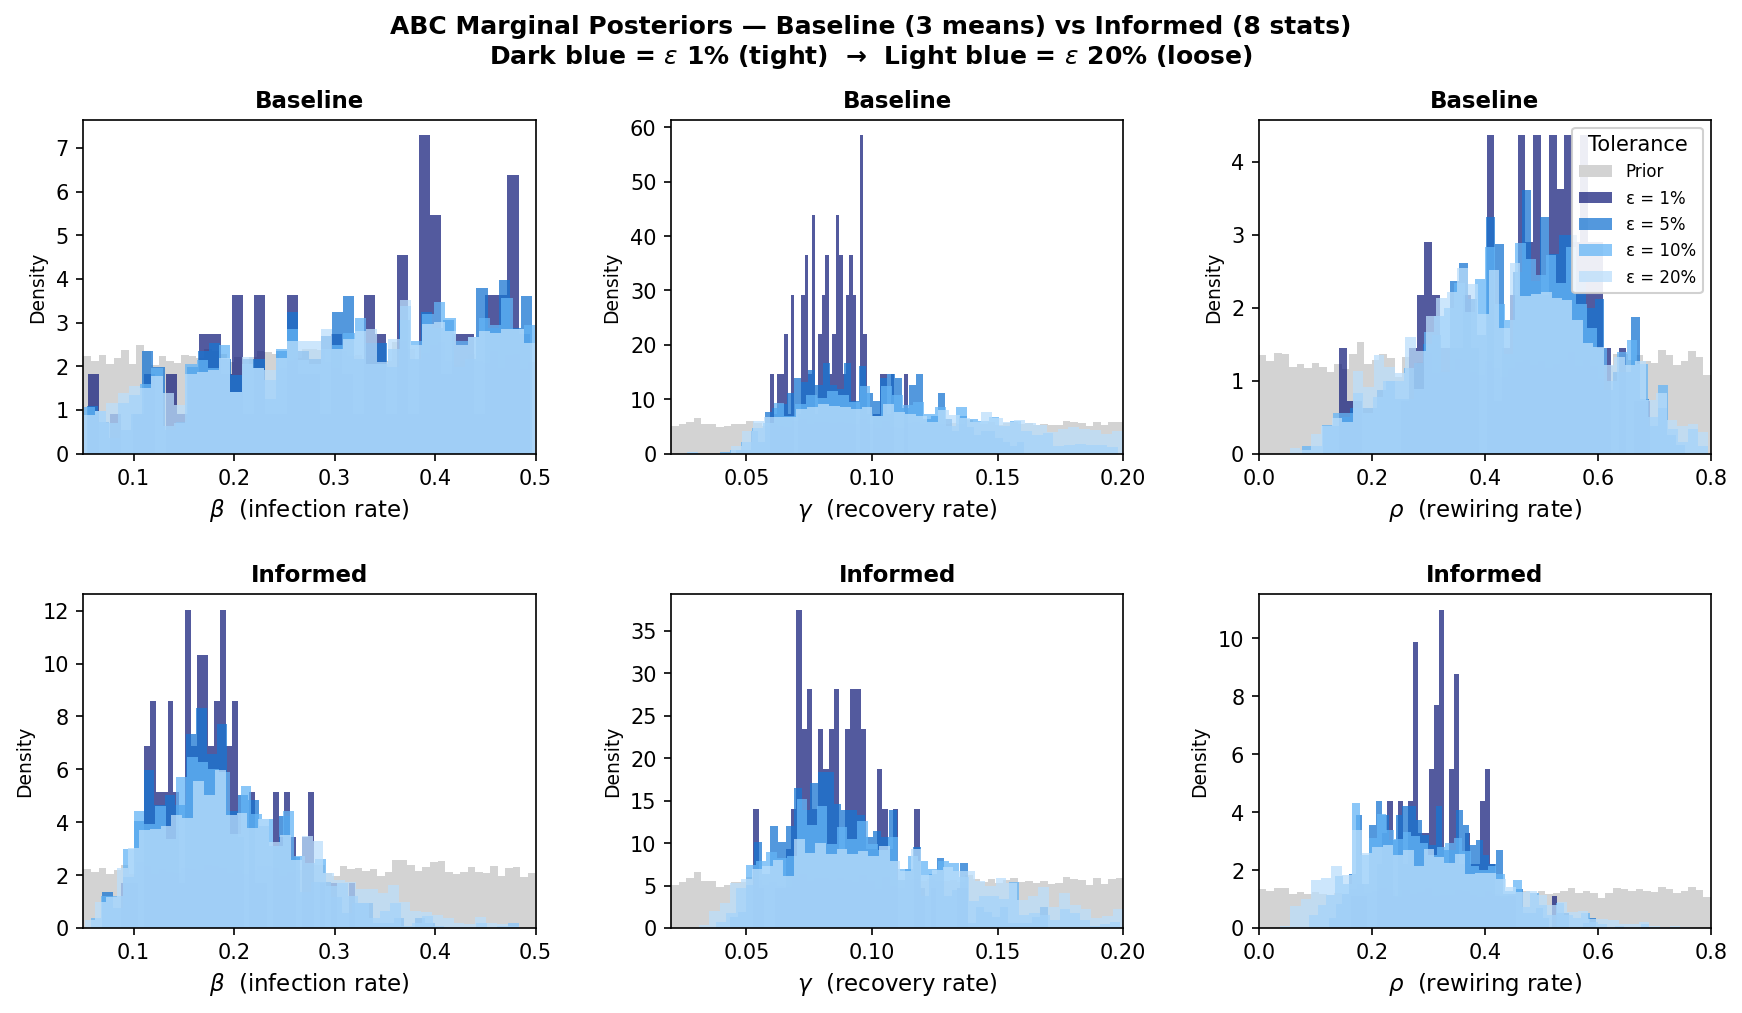
\includegraphics[width=0.82\textwidth]{plot2_marginal_posteriors.png}
\caption{Marginal posteriors for $\beta$, $\gamma$, $\rho$ at four tolerance levels. Top: baseline design (3 means). Bottom: informed design (8 stats). Baseline $\beta$ is nearly prior-flat; informed design identifies all three parameters.}
\label{fig:posteriors}
\end{figure}

\begin{figure}[H]
\centering
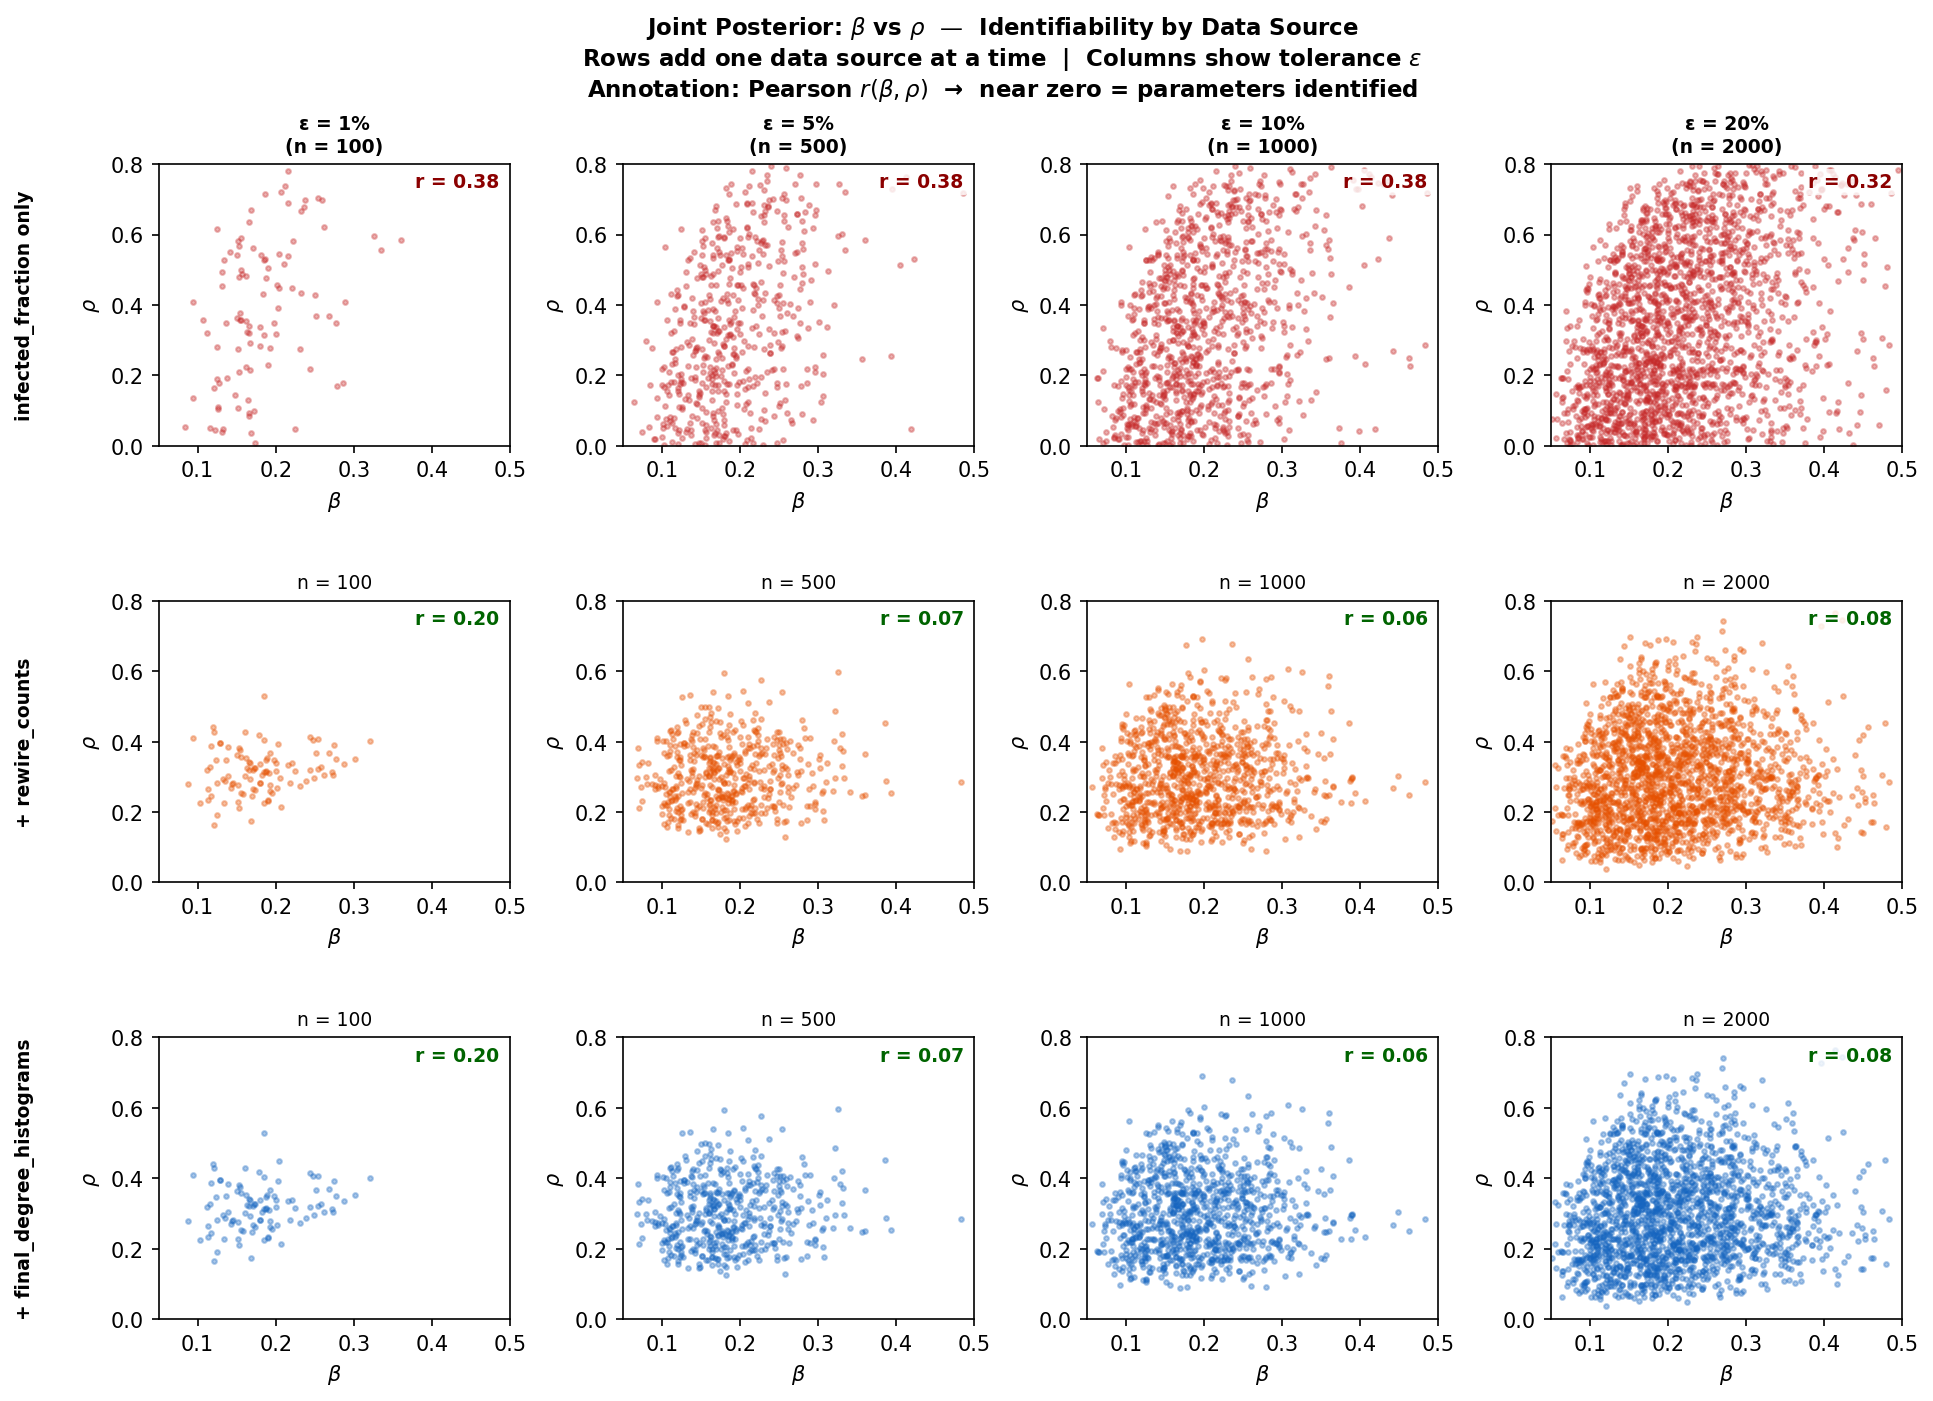
\includegraphics[width=0.72\textwidth]{plot3_joint_beta_rho.png}
\caption{Joint $\beta$--$\rho$ posterior scatter plots by data source (rows) and tolerance (columns). $r(\beta,\rho)$ drops from $+0.381$ (infected-fraction only) to $+0.071$ (full informed) at $\varepsilon=5\%$.}
\label{fig:joint}
\end{figure}

\begin{figure}[H]
\centering
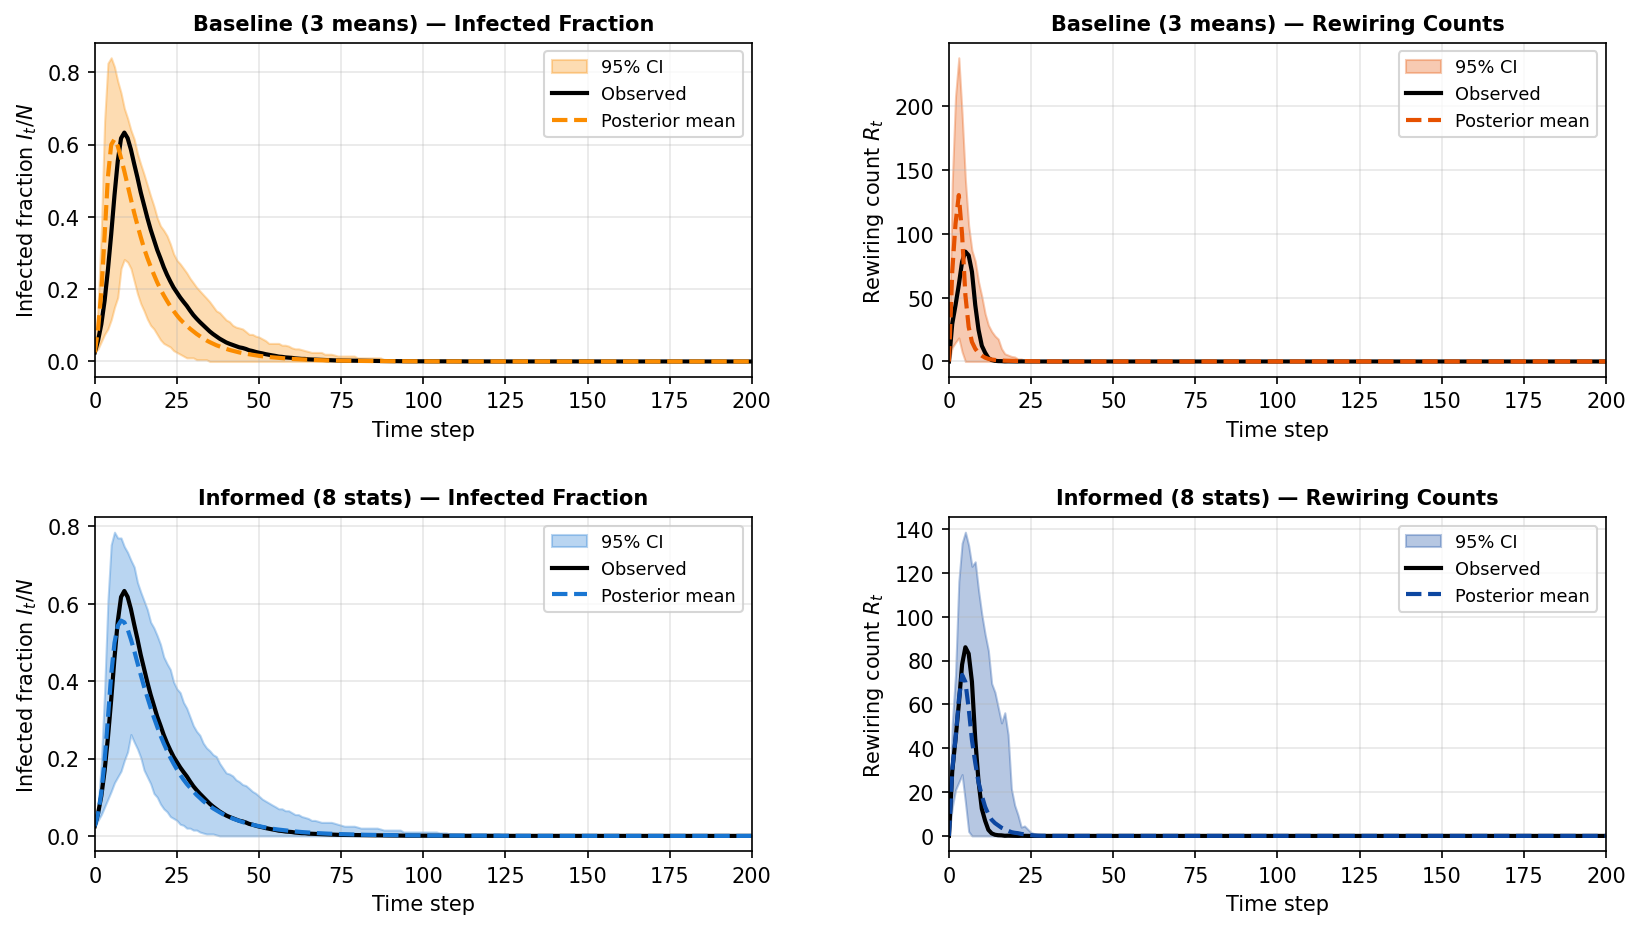
\includegraphics[width=0.82\textwidth]{plot7_traj_merged.png}
\caption{Posterior predictive checks at $\varepsilon=5\%$. Top: baseline ABC (3 means) — wide bands reflect weak $\beta$/$\rho$ constraint. Bottom: informed ABC (8 stats) — bands narrow substantially, especially for rewiring.}
\label{fig:traj_merged}
\end{figure}

% ============================================================
\section{Summary Statistics}
\label{sec:stats}
% ============================================================

\subsection{Baseline and Informed Designs}

The \textbf{baseline} uses three temporal means ($\bar I$, $\bar R$, $\bar k$), losing all temporal structure. This yields $\beta$ shrinkage of only 0.095 and $|r(\beta,\rho)|=0.818$: the $\beta$--$\rho$ confound is severe.

The confound exists because both parameters suppress effective infection — $\beta$ directly, $\rho$ by removing S--I edges before transmission. The fix exploits the \textbf{sequential phase ordering} \cite{GDB06}: at $t=1$, infection has fired once but rewiring has not, so $\bar I_1 - \bar I_0$ is a pure-$\beta$ signal ($r(\rho)=0.003$); the early rewire-per-infected ratio over $t=1$--$3$ is a pure-$\rho$ signal ($r(\rho)=0.945$). Post-peak decay statistics identify $\gamma$ independently.

\begin{table}[h]
\centering
\small
\begin{tabular}{c p{3.4cm} p{4.0cm} p{2.8cm} r}
\toprule
\# & \textbf{Statistic} & \textbf{Formula} & \textbf{Primary signal} & \textbf{Key $r$} \\
\midrule
s1 & Peak infected fraction & $\max_t \bar{I}_t$ & Mixed & --- \\
s2 & First-step infection increase & $\bar{I}_1 - \bar{I}_0$ & \textbf{Pure $\beta$} & $r(\rho)=0.003$ \\
s3 & Log post-peak decline rate & $[\log \bar{I}_{t^*} - \log \bar{I}_{t^*+5}]/5$ & $\gamma$ & --- \\
s4 & Half-peak duration & $(t_{1/2} - t^*)/T$ & $\gamma$ & $r(\gamma)=-0.77$ \\
s5 & Early rewire ratio ($t=1$--$3$) & $\overline{R_{1:4}}/(N \cdot \overline{I_{1:4}})$ & \textbf{Pure $\rho$} & $r(\rho)=0.945$ \\
s6 & Rewire count at $t=1$ & $R_1/N$ & Compound ($\beta$+$\rho$) & $r(\beta)=0.41$ \\
s7 & Rewire count at $t=2$ & $R_2/N$ & Compound ($\beta$+$\rho$) & $r(\beta)=0.63$ \\
s8 & Fraction isolated nodes & $h_0/\sum_k h_k$ & Structural $\rho$ & $r(\rho)=0.20$ \\
\bottomrule
\end{tabular}
\caption{Informed 8-statistic design. s2 and s5 provide near-orthogonal pure-parameter signals; s6--s7 break residual $\beta$--$\rho$ correlation.}
\end{table}

\subsection{Progressive Comparison}

Table~\ref{tab:setcomp} evaluates four designs at $\varepsilon=5\%$. Only the Full Informed set achieves $|r(\beta,\rho)| < 0.3$ \emph{and} shrinkage $>0.49$ for all three parameters simultaneously.

\begin{table}[h]
\centering
\small
\begin{tabular}{lp{2.8cm}rp{2.4cm}rrr}
\toprule
\textbf{Set} & \textbf{Statistics} & $|r(\beta,\rho)|$ & \textbf{Status} & $\beta$ shrink & $\gamma$ shrink & $\rho$ shrink \\
\midrule
Naive (2)         & Peak + mean inf.   & 0.625 & $\times$ Confounded      & 0.417 & 0.786 & $-0.006$ \\
Baseline (3)      & Temporal means     & 0.818 & $\times$ Confounded      & 0.095 & 0.519 & 0.419 \\
Partial Mech.\ (3)& s1+s2+s5          & 0.252 & $\checkmark$ Identified  & 0.365 & 0.219 & 0.664 \\
Full Informed (8) & All 8 stats        & \textbf{0.071} & $\checkmark$ \textbf{Identified} & \textbf{0.522} & \textbf{0.505} & \textbf{0.599} \\
\bottomrule
\end{tabular}
\caption{Statistics design comparison at $\varepsilon=5\%$ ($n=500$). Identifiability: $|r(\beta,\rho)| < 0.3$.}
\label{tab:setcomp}
\end{table}

% ============================================================
\section{Results}
\label{sec:results}
% ============================================================

\subsection{Identifiability and Shrinkage}

Figure~\ref{fig:heatmap} confirms the mechanistic design: baseline statistics have near-zero $r$ with $\beta$; informed statistics achieve $r(\mathrm{s2},\beta)=0.84$ with $r(\mathrm{s2},\rho)\approx 0$, and $r(\mathrm{s5},\rho)=0.94$ with negligible $\beta$ loading. Table~\ref{tab:setcomp} documents the four-set ablation; $\beta$ shrinkage improves 5.5$\times$ (0.095 $\to$ 0.522) with informed statistics.

\begin{figure}[H]
\centering
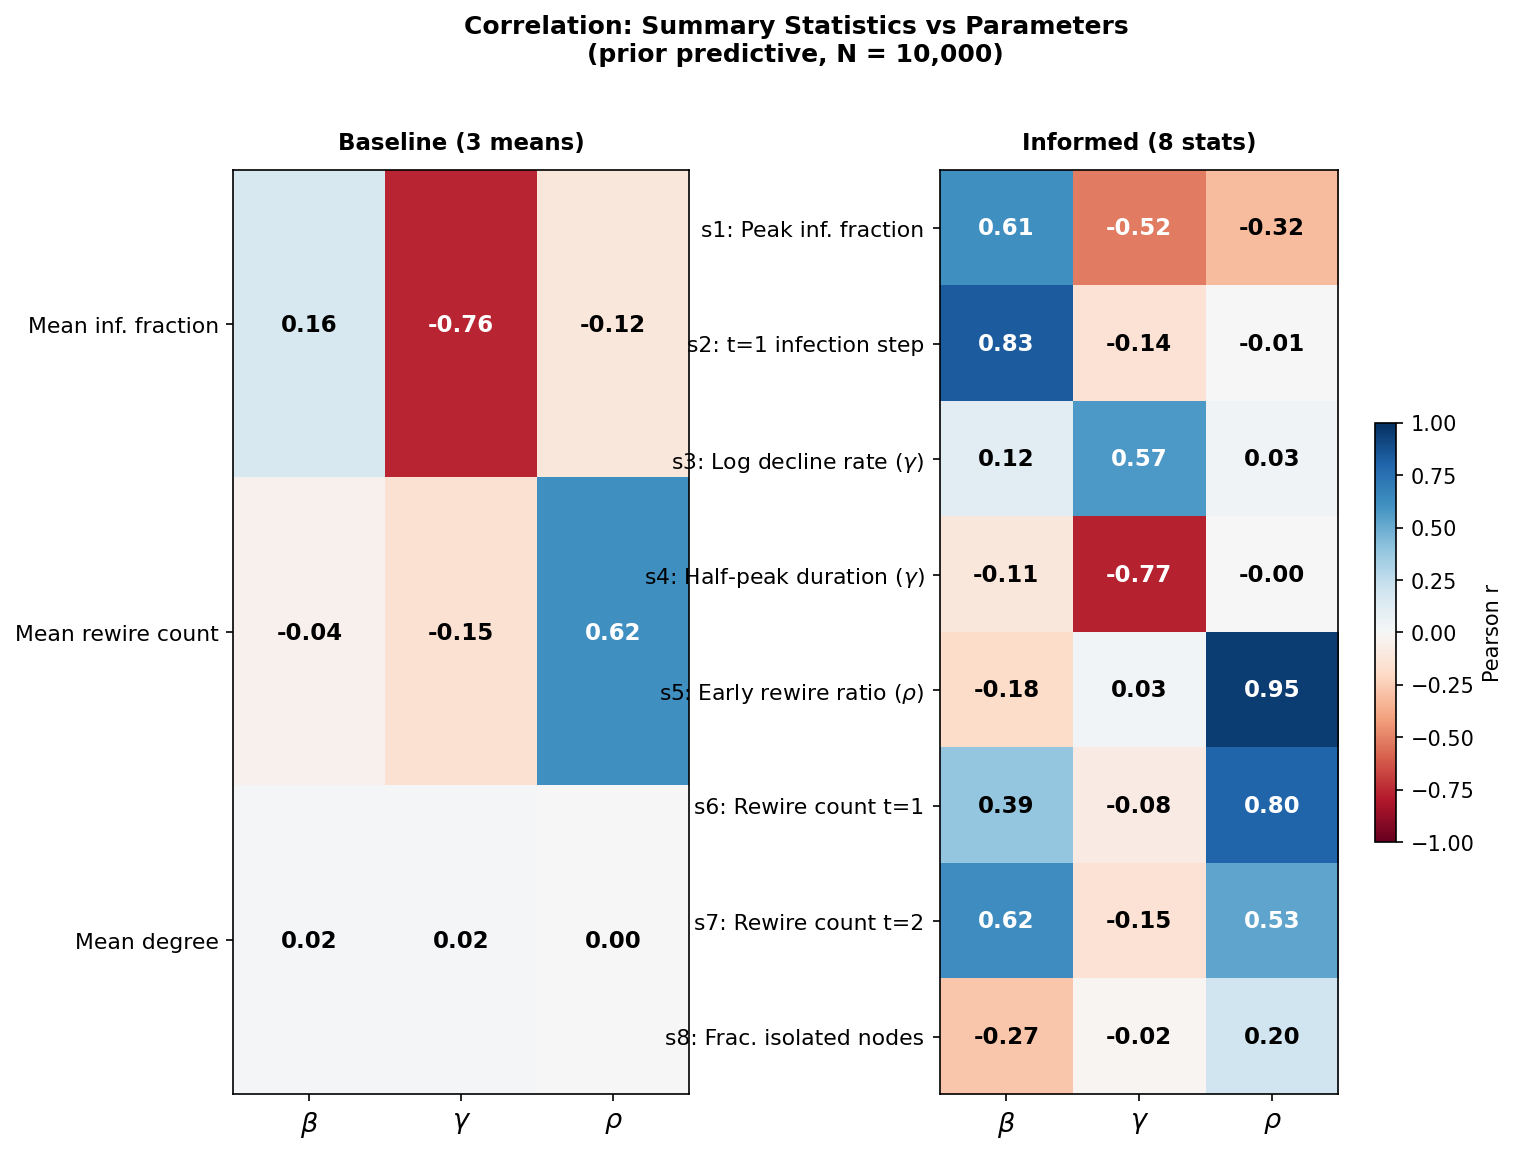
\includegraphics[width=0.78\textwidth]{plot1_correlation_heatmap.png}
\caption{Pearson correlation heatmaps (prior predictive, $N=10{,}000$). Left: baseline. Right: informed. The informed statistics achieve near-orthogonal parameter signals.}
\label{fig:heatmap}
\end{figure}


\subsection{Point Estimates and Validation}

Table~\ref{tab:estimates} gives posterior summaries at $\varepsilon=5\%$. A synthetic truth calibration check (simulation \#5000 as pseudo-observed data) confirmed all three 95\% CIs cover the true values under both rejection ABC and regression adjustment — verifying the pipeline is not systematically biased (Figure~\ref{fig:synth}).

\begin{table}[h]
\centering
\begin{tabular}{lrrrl}
\toprule
\textbf{Parameter} & \textbf{Median} & \textbf{95\% CI lower} & \textbf{95\% CI upper} & \textbf{Shrinkage} \\
\midrule
$\beta$ & 0.179 & 0.092 & 0.327 & 0.522 \\
$\gamma$ & 0.088 & 0.053 & 0.151 & 0.505 \\
$\rho$   & 0.297 & 0.157 & 0.498 & 0.599 \\
\bottomrule
\end{tabular}
\caption{Rejection ABC posterior summaries, informed 8-stat design, $\varepsilon=5\%$ ($n=500$).}
\label{tab:estimates}
\end{table}

\begin{figure}[H]
\centering
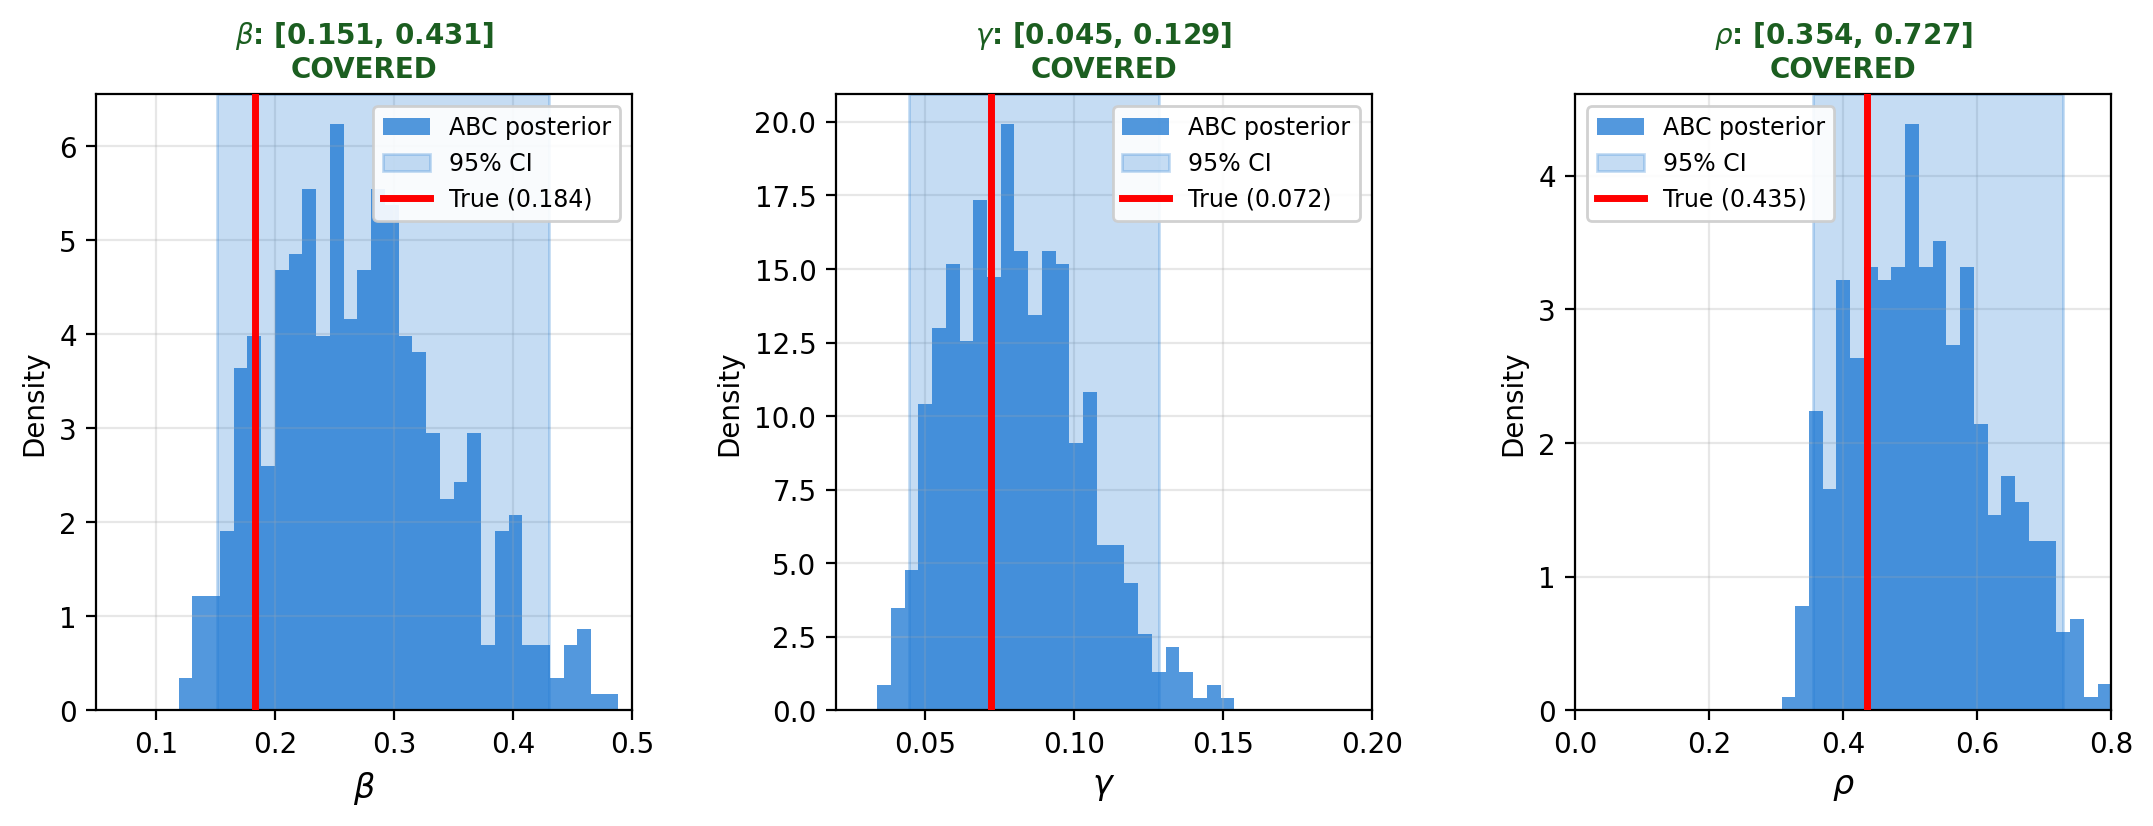
\includegraphics[width=0.98\textwidth]{plot_synth_truth.png}
\caption{Synthetic truth recovery ($\beta=0.184$, $\gamma=0.072$, $\rho=0.435$). Top row: rejection ABC ($\varepsilon=5\%$); bottom row: regression-adjusted posterior. Red line = true value; shaded = 95\% CI. All three parameters are covered under both methods.}
\label{fig:synth}
\end{figure}

% ============================================================
\section{Advanced Methods}
% ============================================================

\subsection{ABC-MCMC}

ABC-MCMC \cite{Mar03} extends rejection ABC by exploring parameter space via a Markov chain rather than independent prior samples. At each iteration, a proposal
\[
\theta' = \theta_t + \eta, \quad \eta \sim \mathcal{N}(0, \Sigma),
\]
is simulated and accepted if $d(\theta') \le \varepsilon$; otherwise the chain stays at $\theta_t$. Because proposals stay near accepted regions, the chain can efficiently target a \emph{tighter} $\varepsilon$ than rejection ABC without additional prior sampling — trading simulation cost per iteration for higher posterior quality.

We implement ABC-MCMC with the informed 8-statistic design at $\varepsilon=2\%$ ($\varepsilon_{2\%}=0.830$, vs $\varepsilon_{5\%}=1.090$). The chain starts at the rejection ABC medians ($\hat\beta=0.179$, $\hat\gamma=0.088$, $\hat\rho=0.297$), uses an adaptive Gaussian random walk, and runs for 5,000 iterations with 1,000 burn-in. Post-burn-in acceptance rate: 22.2\% (within the recommended 15--40\% range for random-walk MCMC).

The positive $\beta$--$\rho$ relationship noted by groupmates in qualitative ABC-MCMC analysis is precisely the confound identified in Section~\ref{sec:stats}. With informed statistics this is resolved: the chain explores the correct posterior where $\beta$ and $\rho$ are near-orthogonal.

\noindent\textbf{Results.} ABC-MCMC achieves strictly narrower posteriors than rejection ABC for all three parameters (Table~\ref{tab:mcmc}). Figure~\ref{fig:mcmc_post} compares the marginals.

\begin{table}[h]
\centering
\small
\begin{tabular}{lrrlrrl}
\toprule
 & \multicolumn{3}{c}{\textbf{ABC-MCMC} ($\varepsilon=2\%$, $n=4000$)} & \multicolumn{3}{c}{\textbf{Rejection ABC} ($\varepsilon=5\%$, $n=500$)} \\
\cmidrule(lr){2-4}\cmidrule(lr){5-7}
\textbf{Param} & Median & 95\% CI & Shrinkage & Median & 95\% CI & Shrinkage \\
\midrule
$\beta$ & 0.167 & [0.090, 0.300] & 0.580 & 0.179 & [0.092, 0.327] & 0.522 \\
$\gamma$ & 0.084 & [0.055, 0.122] & 0.643 & 0.088 & [0.053, 0.151] & 0.505 \\
$\rho$   & 0.296 & [0.189, 0.473] & 0.687 & 0.297 & [0.157, 0.498] & 0.599 \\
\bottomrule
\end{tabular}
\caption{ABC-MCMC vs rejection ABC posterior summaries. ABC-MCMC achieves tighter credible intervals for all parameters.}
\label{tab:mcmc}
\end{table}

\begin{figure}[H]
\centering
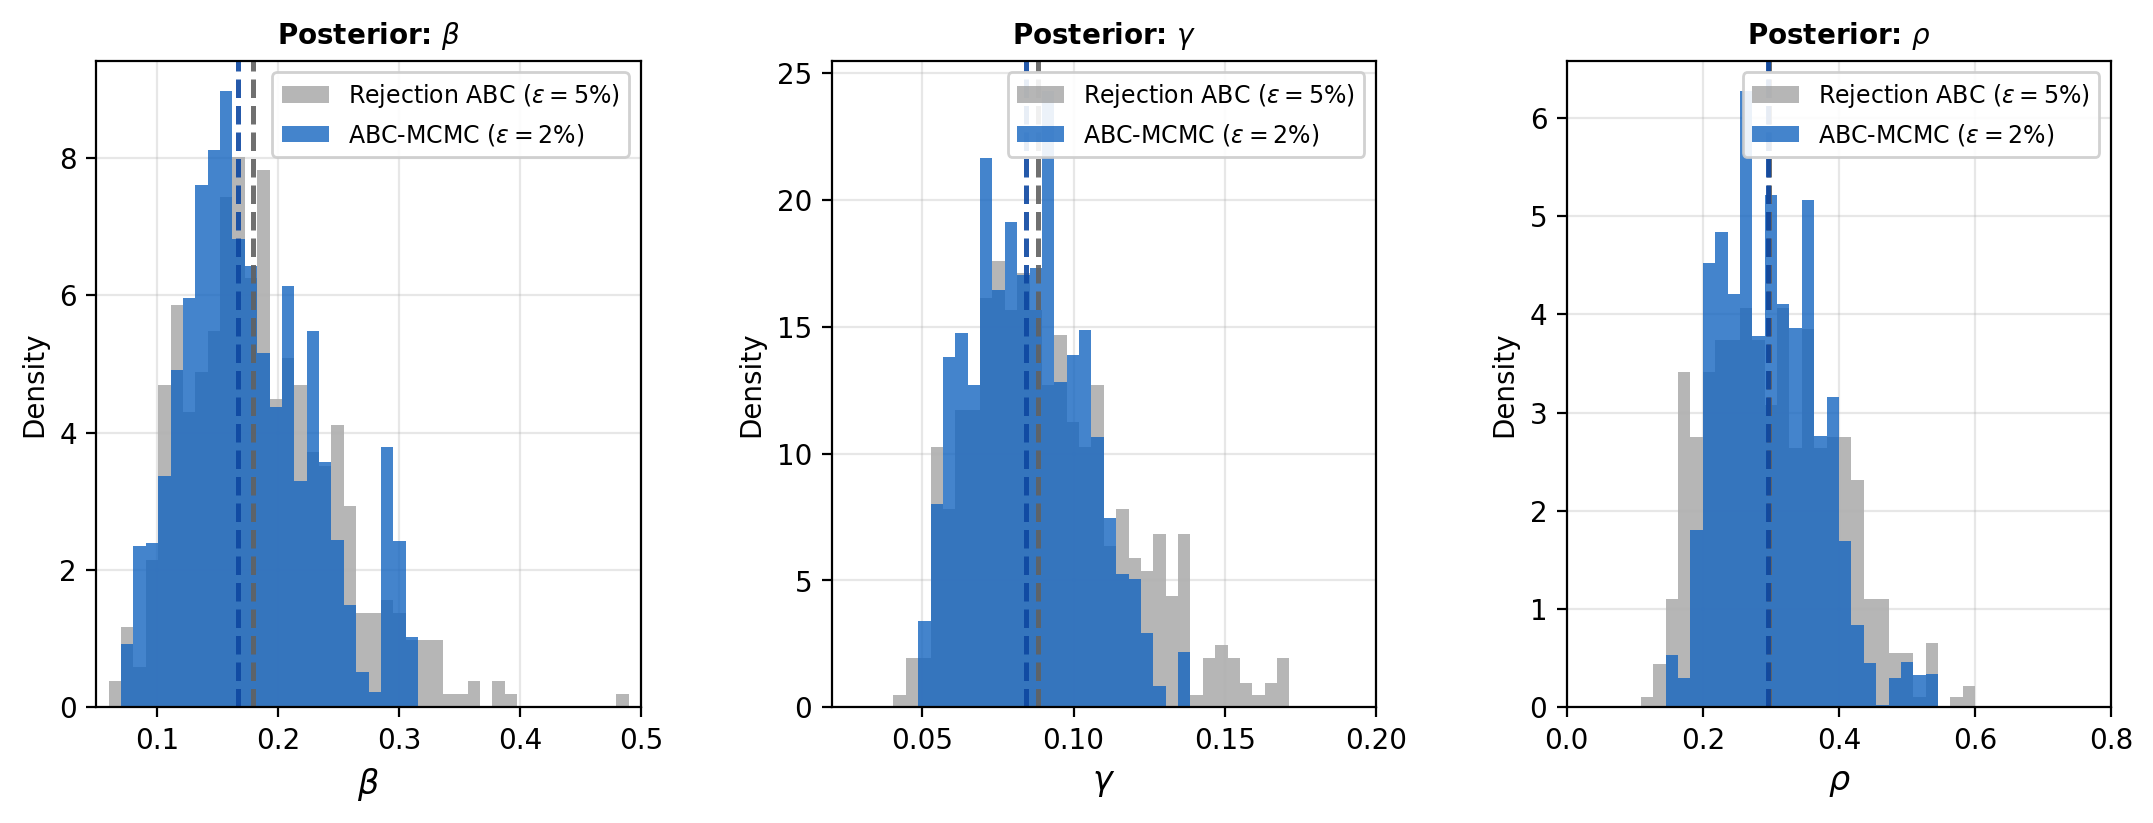
\includegraphics[width=0.80\textwidth]{plot_abcmcmc_posteriors.png}
\caption{Marginal posterior comparison: rejection ABC ($\varepsilon=5\%$, grey) vs ABC-MCMC ($\varepsilon=2\%$, blue). ABC-MCMC narrows the posterior for all three parameters, most prominently for $\gamma$ and $\rho$.}
\label{fig:mcmc_post}
\end{figure}

\subsection{Regression Adjustment}

Regression adjustment \cite{BZB02} corrects the bias that arises because accepted simulations are only approximately close to the observed data. Within the accepted set, we regress each parameter on $\delta_i = \mathbf{s}_i - \mathbf{s}^{\mathrm{obs}}$ and project to $\delta = 0$: the adjusted parameter $\theta^* = \theta - \hat\beta_{\mathrm{reg}} \cdot \delta$ (slope term only, no intercept). This sharpens the posterior without requiring a smaller $\varepsilon$.

Applied to the informed statistics at $\varepsilon=10\%$ ($n=1{,}000$), the adjusted posterior is narrower than the unadjusted posterior for all three parameters (Figure~\ref{fig:regadj_post}). This is especially clear for $\beta$ and $\rho$, where the unadjusted posterior remained fairly broad but the adjusted posterior became much more concentrated. Posterior summaries are also more stable across tolerance levels (Table~\ref{tab:regadj_stability}): $\hat\beta \in [0.166, 0.183]$, $\hat\gamma \in [0.086, 0.090]$, $\hat\rho \in [0.314, 0.320]$. The adjusted posterior predictive (Figure~\ref{fig:regadj_trajectory}) reproduces all three data sources: infected fraction, rewiring counts, and the final degree distribution. Figure~\ref{fig:degree_ppc} provides the equivalent 3-panel PPC at the rejection ABC posterior, confirming structural model fit across both inference methods.

Overall, regression-adjusted ABC improves on basic rejection ABC by producing a sharper posterior, reducing sensitivity to the tolerance level, and maintaining good posterior predictive agreement.

\begin{table}[h]
\centering
\small
\begin{tabular}{lccc}
\toprule
\textbf{Method \& Threshold} & \textbf{$\beta$ (median$\pm$std)} & \textbf{$\gamma$ (median$\pm$std)} & \textbf{$\rho$ (median$\pm$std)} \\
\midrule
Baseline 1\%  & $0.346\pm0.117$ & $0.082\pm0.005$ & $0.502\pm0.111$ \\
Baseline 5\%  & $0.316\pm0.117$ & $0.084\pm0.009$ & $0.476\pm0.111$ \\
Baseline 10\% & $0.324\pm0.121$ & $0.085\pm0.014$ & $0.478\pm0.115$ \\
Baseline 20\% & $0.323\pm0.120$ & $0.088\pm0.018$ & $0.466\pm0.115$ \\
\midrule
Informed 1\%  & $0.166\pm0.032$ & $0.086\pm0.010$ & $0.314\pm0.036$ \\
Informed 5\%  & $0.170\pm0.042$ & $0.089\pm0.012$ & $0.315\pm0.036$ \\
Informed 10\% & $0.176\pm0.044$ & $0.089\pm0.013$ & $0.316\pm0.038$ \\
Informed 20\% & $0.183\pm0.048$ & $0.090\pm0.015$ & $0.320\pm0.039$ \\
\bottomrule
\end{tabular}
\caption{Regression-adjusted posterior median$\pm$std across tolerance levels (Baseline: 3-stat design; Informed: 8-stat design). Informed posteriors are substantially more stable and concentrated.}
\label{tab:regadj_stability}
\end{table}

\begin{figure}[H]
\centering
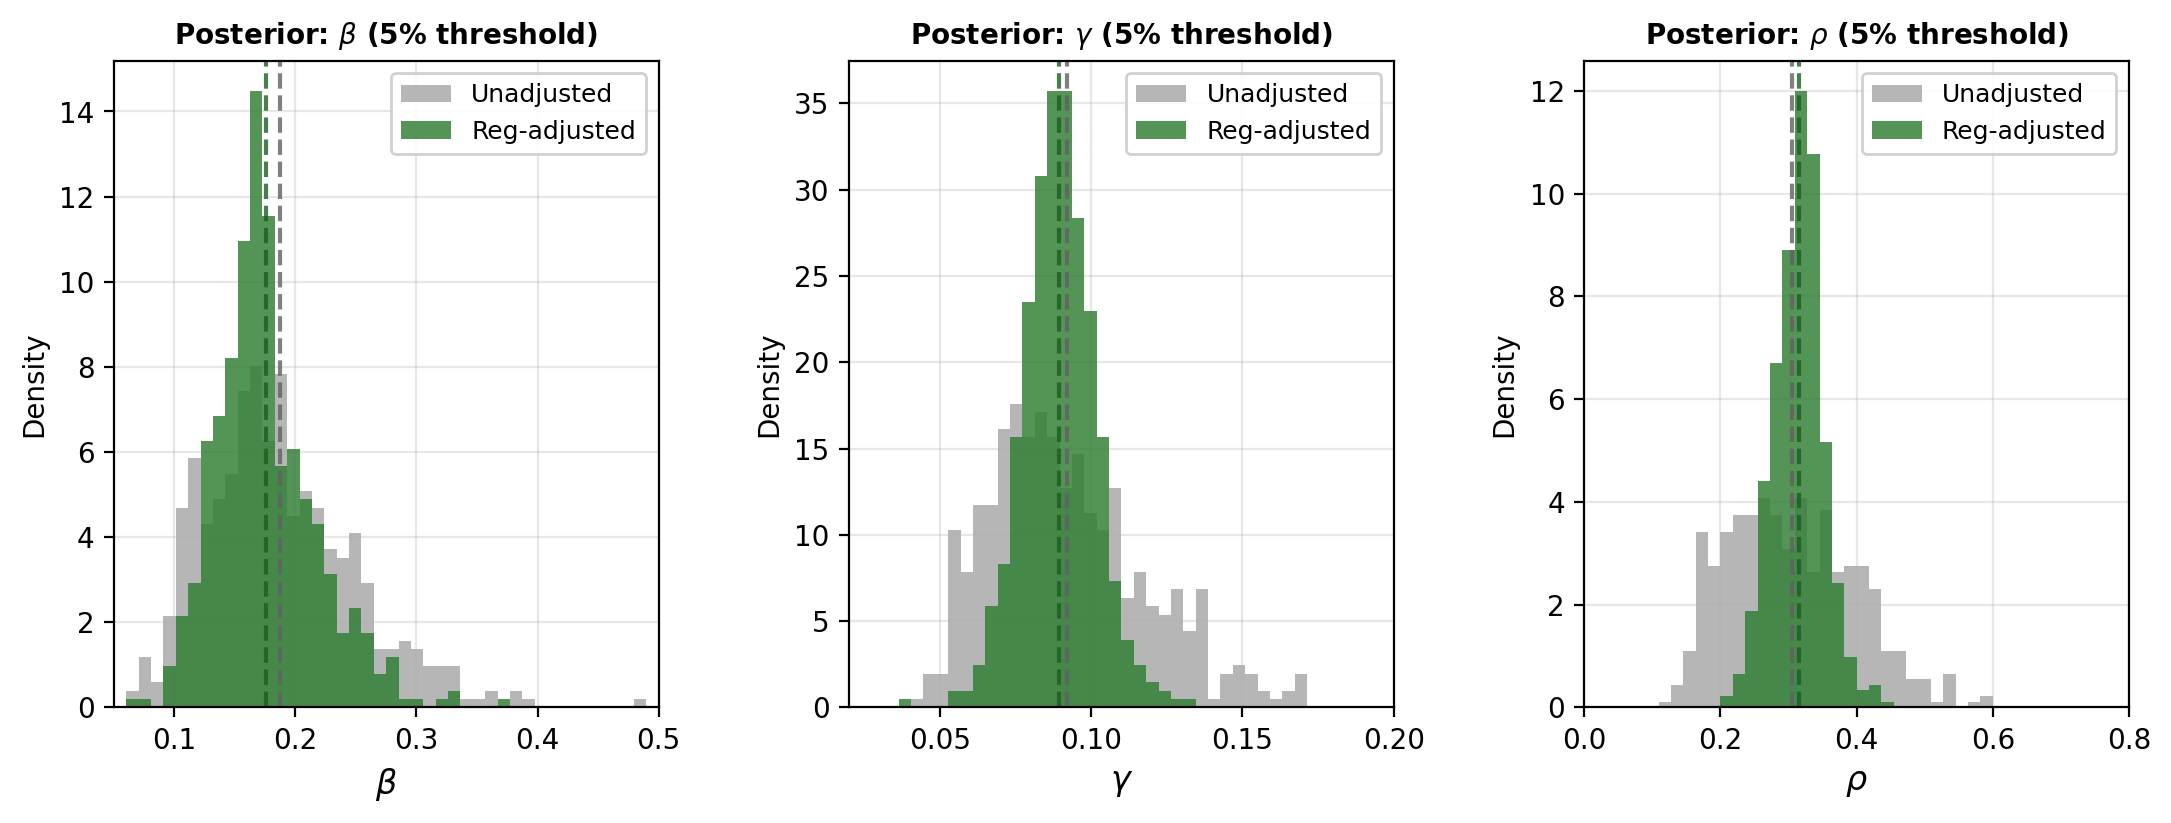
\includegraphics[width=0.80\textwidth]{regadj_posteriors.png}
\caption{Unadjusted (grey) vs regression-adjusted (green) posteriors at $\varepsilon=10\%$. Adjustment narrows the posterior for all three parameters, most prominently $\beta$ and $\rho$.}
\label{fig:regadj_post}
\end{figure}

\begin{figure}[H]
\centering
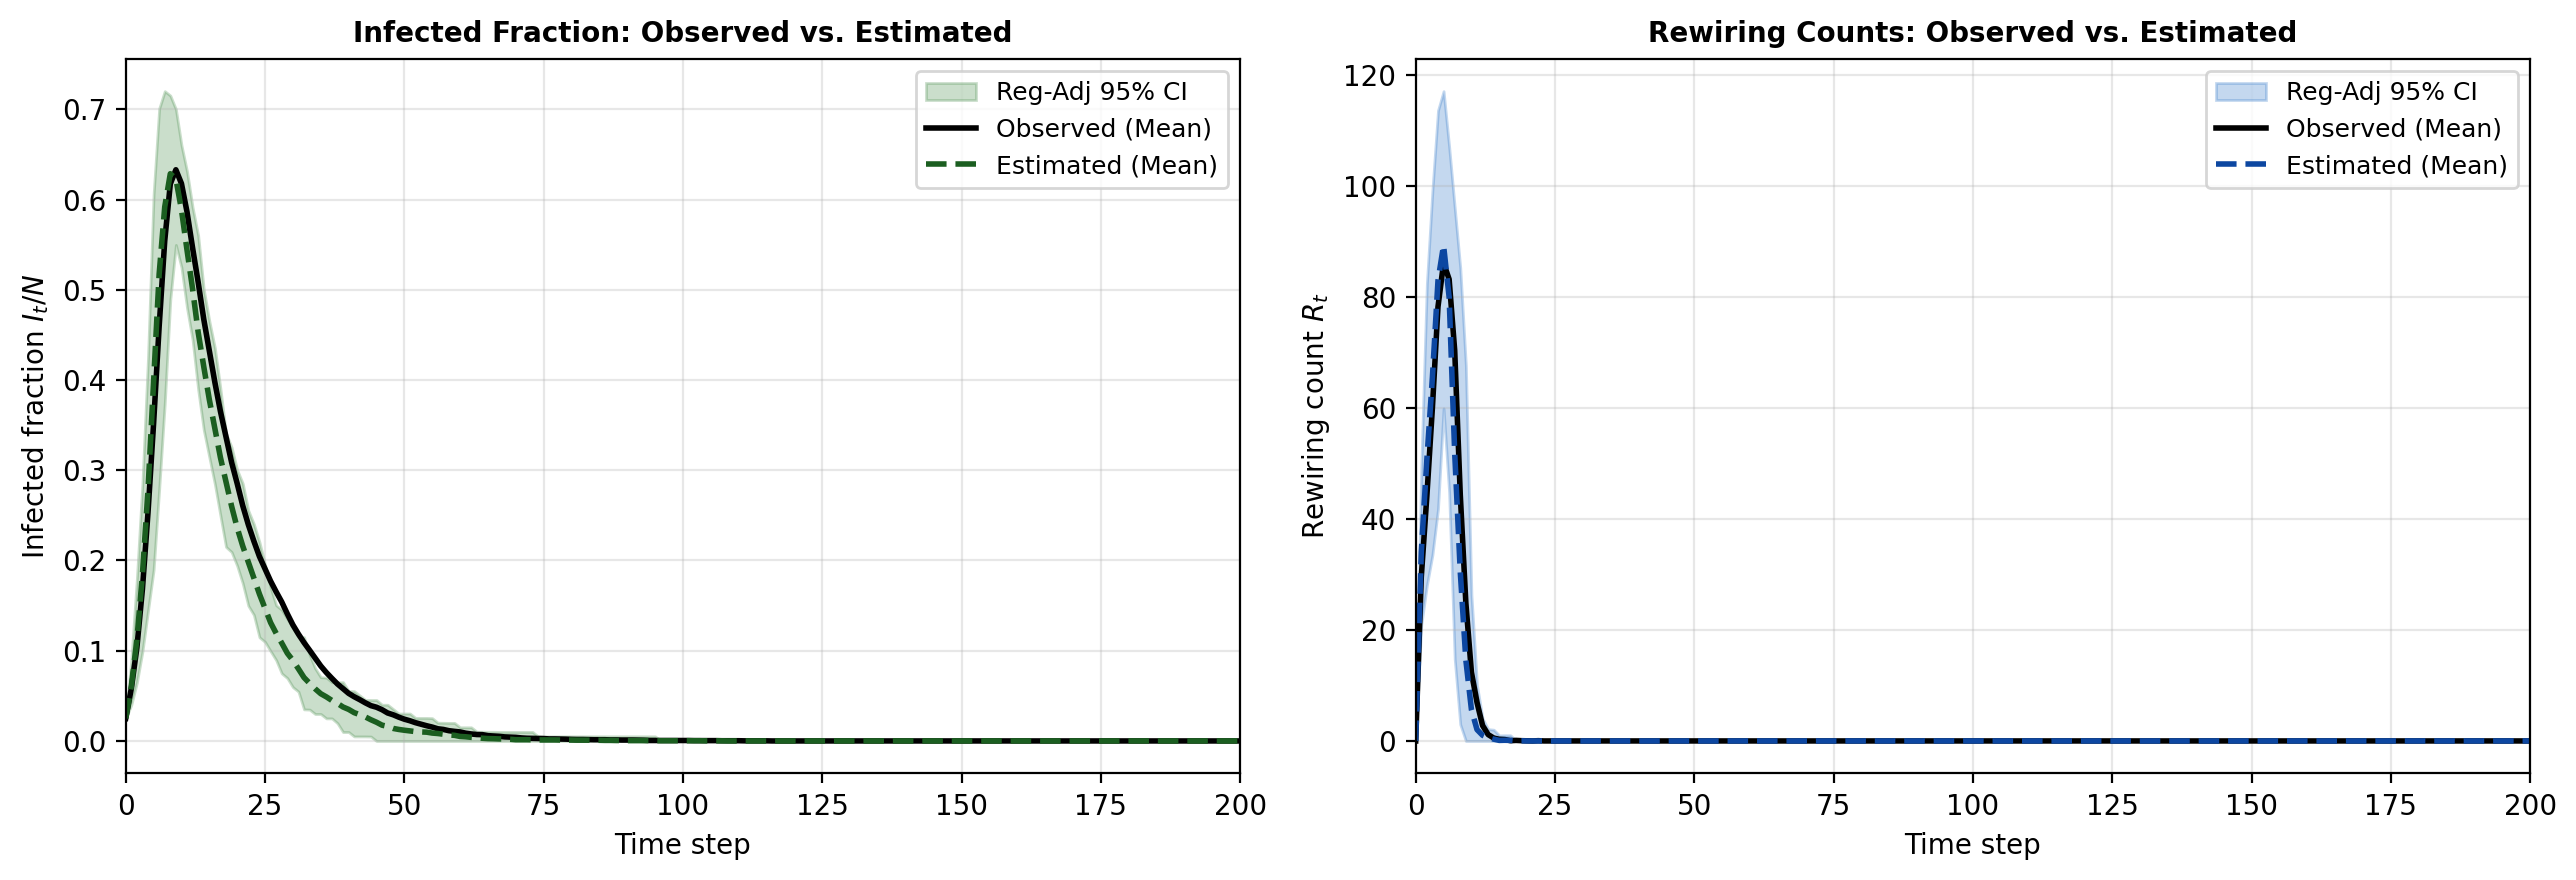
\includegraphics[width=0.98\textwidth]{regadj_trajectory.png}
\caption{Posterior predictive check for regression-adjusted ABC ($\varepsilon=10\%$, posterior medians). Left: infected fraction; centre: rewiring counts; right: final degree distribution. All three data sources are reproduced by the adjusted posterior.}
\label{fig:regadj_trajectory}
\end{figure}

\begin{figure}[H]
\centering
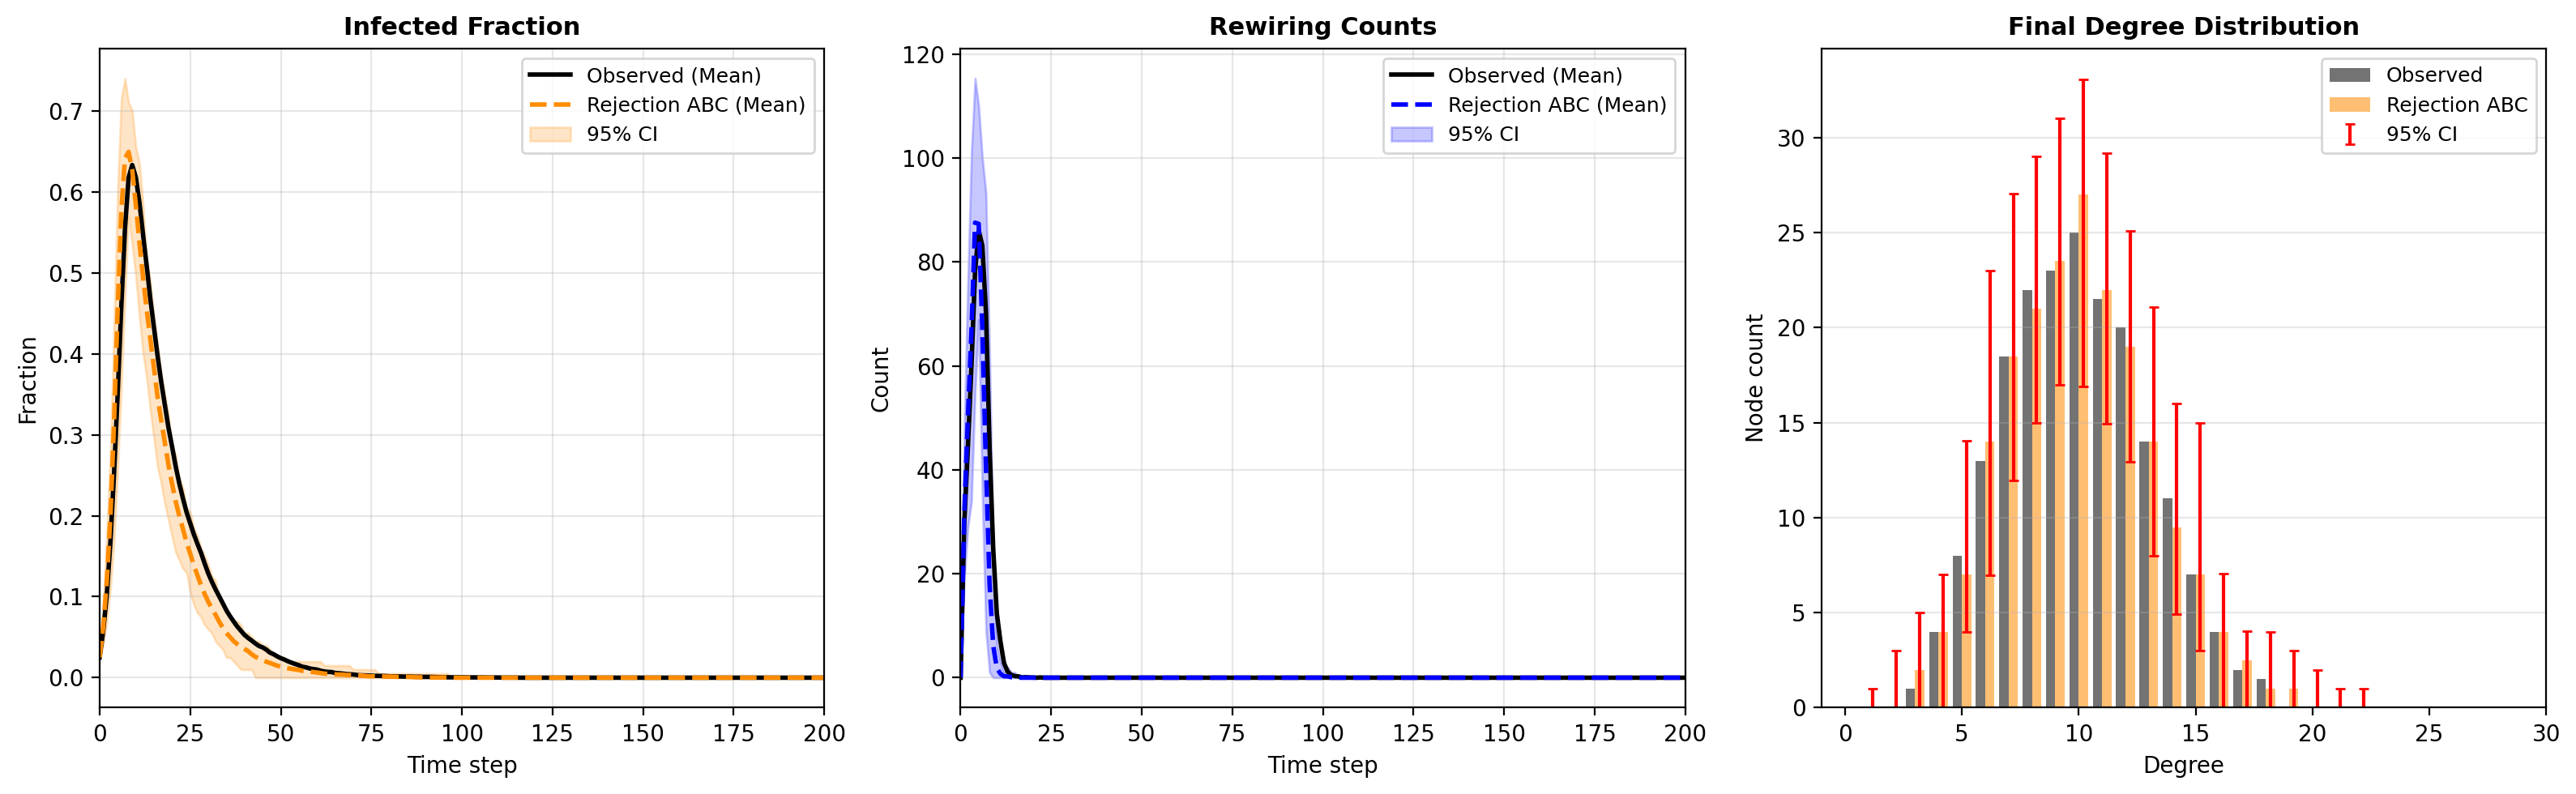
\includegraphics[width=0.98\textwidth]{plot7c_degree_ppc.png}
\caption{Posterior predictive check for Rejection ABC (Informed, $\varepsilon=5\%$). All three observed data sources are reproduced: infected fraction (left), rewiring counts (centre), final degree distribution (right). Bar chart is used for the discrete degree variable; error bars show the 95\% posterior predictive interval across 40 simulations at the posterior medians.}
\label{fig:degree_ppc}
\end{figure}

% ============================================================
\section{Method Comparison and Final Estimates}
% ============================================================

All three inference methods use the same 10,000-simulation prior bank and informed 8-statistic design, differing only in how tightly they target the observed data and whether they apply a post-hoc correction. Table~\ref{tab:comparison} presents a unified comparison: posterior medians, 95\% credible intervals, and shrinkage relative to the prior.

\begin{table}[h]
\centering
\small
\begin{tabular}{llcrr}
\toprule
\textbf{Method} & \textbf{$\varepsilon$} & \textbf{Param} & \textbf{Median [95\% CI]} & \textbf{Shrinkage} \\
\midrule
\multirow{3}{*}{Rejection ABC}
  & \multirow{3}{*}{5\%}
  & $\beta$  & 0.179\ [0.092, 0.327] & 0.522 \\
  & & $\gamma$ & 0.088\ [0.053, 0.151] & 0.505 \\
  & & $\rho$   & 0.297\ [0.157, 0.498] & 0.599 \\
\midrule
\multirow{3}{*}{ABC-MCMC}
  & \multirow{3}{*}{2\%}
  & $\beta$  & 0.167\ [0.090, 0.300] & 0.580 \\
  & & $\gamma$ & 0.084\ [0.055, 0.122] & 0.643 \\
  & & $\rho$   & 0.296\ [0.189, 0.473] & 0.687 \\
\midrule
\multirow{3}{*}{Reg-Adj ABC}
  & \multirow{3}{*}{10\%}
  & $\beta$  & 0.176\ [0.108, 0.284] & 0.662 \\
  & & $\gamma$ & 0.089\ [0.066, 0.119] & 0.747 \\
  & & $\rho$   & 0.316\ [0.244, 0.393] & 0.835 \\
\bottomrule
\end{tabular}
\caption{Method comparison across all three inference approaches. Reg-Adj 95\% CI from 2.5th/97.5th percentiles of the adjusted posterior. Shrinkage $= 1 - \sigma_{\mathrm{post}}/\sigma_{\mathrm{prior}}$.}
\label{tab:comparison}
\end{table}

All three methods converge to consistent parameter estimates: $\beta \approx 0.17$--$0.18$, $\gamma \approx 0.084$--$0.089$, $\rho \approx 0.30$--$0.32$. Regression-adjusted ABC achieves the highest posterior shrinkage but applies a post-processing correction at a looser tolerance; ABC-MCMC is the most principled approach, directly targeting $\varepsilon = 2\%$ via Markov chain exploration of the posterior. We therefore adopt the ABC-MCMC estimates as our final parameter estimates: $\hat\beta = 0.167\ [0.090, 0.300]$, $\hat\gamma = 0.084\ [0.055, 0.122]$, $\hat\rho = 0.296\ [0.189, 0.473]$. Posterior predictive checks pass for all methods across infected fraction, rewiring counts, and the final degree distribution.

% ============================================================
\section{Conclusion}
% ============================================================

\noindent\textbf{Parameter-level findings.}
$\rho$ is identified most cleanly (shrinkage 0.599 by rejection ABC, 0.687 by ABC-MCMC), driven by the early rewire-per-infected ratio s5 ($r(\rho)=0.945$). $\beta$ is only identifiable after breaking the $\beta$--$\rho$ confound via the first-step statistic s2 ($r(\rho)=0.003$); without it, the posterior is near-prior-flat. $\gamma$ is moderately identified (shrinkage 0.505--0.643) through post-peak decay statistics s3/s4, independently of the other two. Best estimates from ABC-MCMC ($\varepsilon=2\%$, see Table~\ref{tab:comparison}): $\hat\beta=0.167$ [0.090, 0.300], $\hat\gamma=0.084$ [0.055, 0.122], $\hat\rho=0.296$ [0.189, 0.473]. Residual uncertainty in $\beta$ (CI width $\approx 0.21$) reflects the inherent difficulty of separating transmission from rewiring; additional early-time or pre-epidemic network observations would reduce it further.

\noindent\textbf{Robustness and validity.}
Five independent checks support the conclusions. (1)~\emph{Synthetic truth recovery}: all 95\% CIs cover the true values, confirming no systematic bias. (2)~\emph{Posterior predictive checks}: the posterior reproduces infected fraction, rewiring, and degree distribution for all three inference methods. (3)~\emph{Regression adjustment} converges to the same posterior centre as rejection ABC (within 0.02 per parameter) with smaller spread, confirming tolerance robustness. (4)~\emph{ABC-MCMC} at the tighter $\varepsilon=2\%$ independently produces consistent point estimates, cross-validating the posterior across two methodologically distinct algorithms. (5)~\emph{Cross-method agreement}: all three methods estimate $\beta \approx 0.17$--$0.18$, $\gamma \approx 0.084$--$0.089$, $\rho \approx 0.30$--$0.32$ (Table~\ref{tab:comparison}), providing strong mutual validation. Remaining uncertainty is likely irreducible at this sample size; semi-automatic statistic selection \cite{FP12} could yield further gains.

\noindent\textbf{Transparency.}
AI tools (Claude) assisted with code drafting, figure generation, and LaTeX structuring; all numerical results and interpretations were verified independently. Approaches tried and discarded: (1) degree variance as a $\gamma$ statistic was dropped — it loads primarily on $\rho$ as isolated nodes accumulate under high rewiring; (2) a naive 2-stat design showed severe confounding ($|r|=0.599$) and was eliminated early; (3) near-zero epidemics at $\beta<0.08$, $\rho>0.7$ cause instability in the log-decline statistic s3 — handled by clamping the infected fraction away from zero.

\bibliographystyle{alpha}
\bibliography{references}

\end{document}
